\documentclass{standalone}
\usepackage{tikz}
\usetikzlibrary{automata, positioning}

\begin{document}

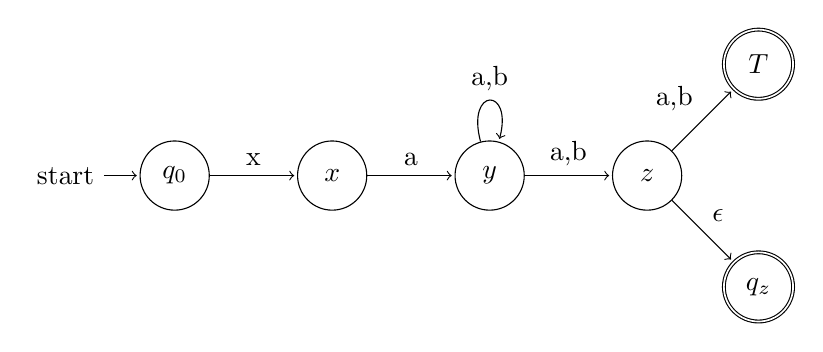
\begin{tikzpicture}[shorten >=1pt, node distance=2cm, on grid, auto] 

  % States
  \node[state, initial] (q0) {$q_0$}; 
  \node[state] (x) [right=of q0] {$x$}; 
  \node[state] (y) [right=of x] {$y$}; 
  \node[state] (z) [right=of y] {$z$}; 
  \node[state, accepting] (qz) [below right=of z] {$q_z$}; 
  \node[state, accepting] (T) [above right=of z] {$T$}; 
  
  % Transitions
  \path[->] 
    (q0) edge node {x} (x)
    (x) edge node {a} (y)
    (y) edge [loop above] node {a,b} (y)
    (y) edge node {a,b} (z)
    (z) edge node {$\epsilon$} (qz)
    (z) edge node {a,b} (T);
  
\end{tikzpicture}

\end{document}
